\chapter[量子もつれ]
{量子もつれ}

\section{CHSHゲーム}
lesson4エンタングルメント(量子もつれ)。このレッスン
ではまずはちょっとゲームを例として量子エンタングルメントのまあバリューとしてお話しますけれどもその後もうちょっと定量的にエンタングルメントの状態を説明してそれから特別な状態bell stateとかについてはお話しするんですけれども最後には量子
ネットワーク量子通信としては量子エンタングルメントを資源として使うことを説明します。


まずはステップ1。CHSHゲーム。このゲームにはプレーヤーが2人
と審判は一人なんですけれどもこの二人AさんとBさんは協力して
レフリーと対局してそれが勝負になります:
% game diagram
\begin{figure}[H]
    \centering
    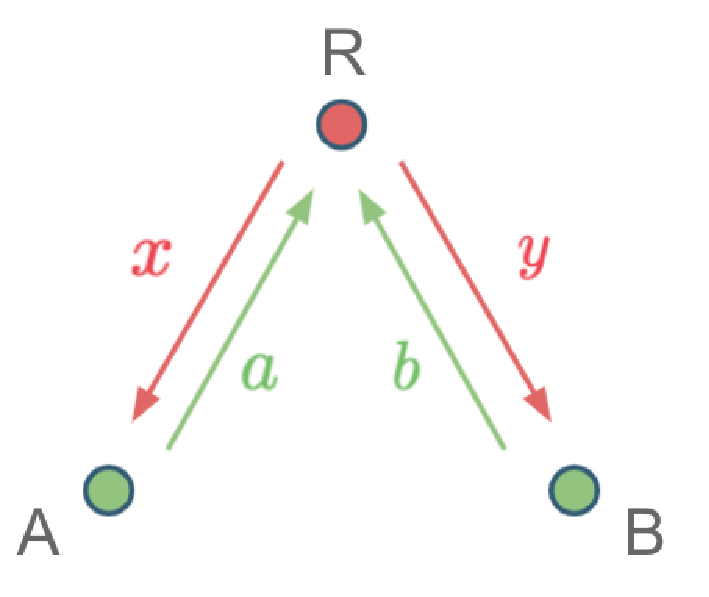
\includegraphics[width=0.5\textwidth]{lesson4/CHSH_diagram.pdf}
    \label{fig: 1}
    \begin{center}
        \caption{CHSHゲーム画像}
    \end{center}
\end{figure}
じゃあちょっとルールを説明します。
\begin{enumerate}
    \item 例えばこの設定でレフリーは上のRのところでAとBさんは下のところですけれどもレフリーが2つの古典ビットをランダムに選択
してそれが$0$か$1$か50-50の確率であります。けれどもそれが$x$と$y$とよんでそれがAさんとBさんに送ります。
    \item AさんとBさんは自分の古典ビットを決めて小文字のaとbとよんで、それを決めてレフリーさんに戻します。審判さんに送る。
    \item ゲームが始まってからAさんとBさんはメッセージを交換するのは
禁止。
\end{enumerate}
勝ち、勝負が\textbf{$x y = a \oplus b$の場合にはプレーヤーの勝ちです}。

じゃあ例を見てみましょう:
% Round 1/2/3 pic
\begin{figure}[H]
    \centering
    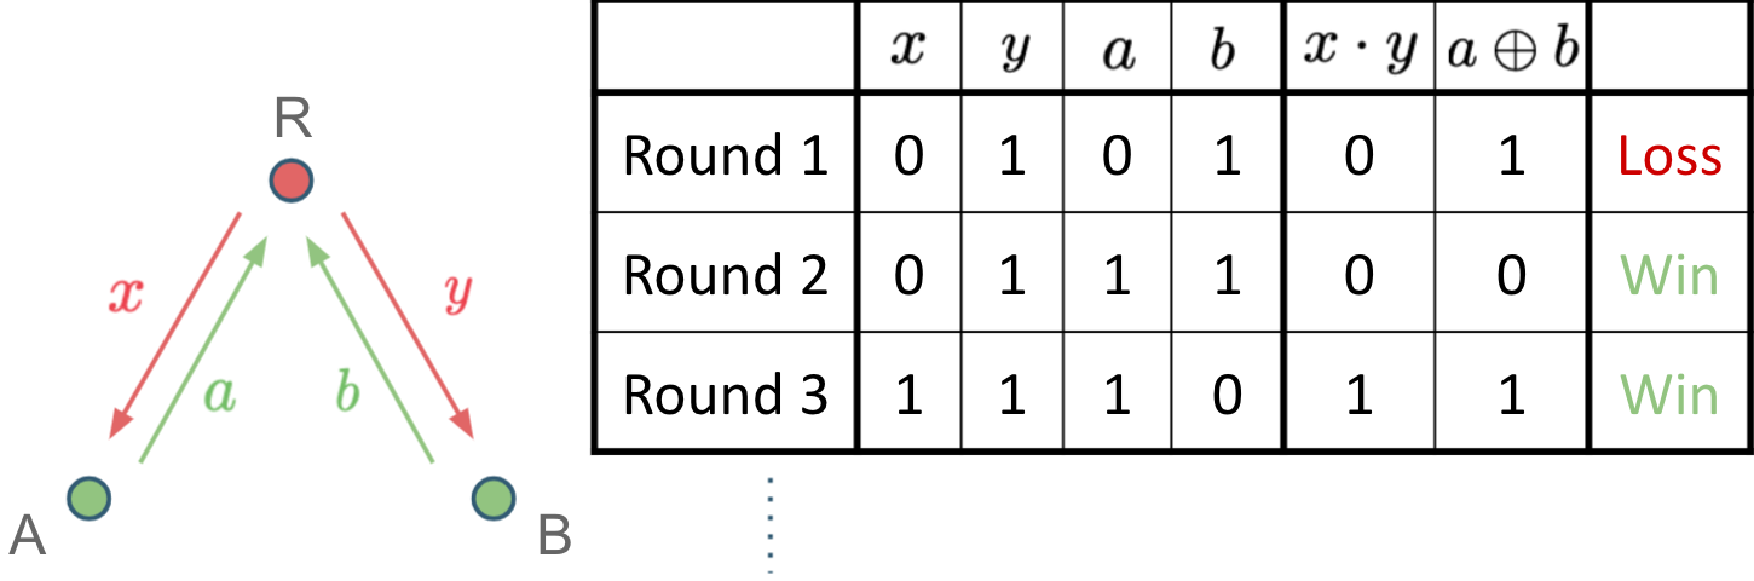
\includegraphics[width=0.8\textwidth]{lesson4/CHSH_rounds.pdf}
    \label{fig: 1}
    \begin{center}
        \caption{CHSHゲームプレイ例}
    \end{center}
\end{figure}
\begin{enumerate}
    \item 、審判さんレフリーがxとyを0と1に決まる場合を見てみましょう(round 1)。$x y = 0$そしてAさんとBさんの目的は$a \oplus b = 0$目標なん
ですけれどもAさんとBさんは0と1に選ぶ場合には、$a \oplus b = 1$で
AさんとBさんの負け。プレーヤー側のゲームは、このラウンドで負けました。
    \item ラウンド2としては、まあ審判さんは0と1を選択するまま、AさんとBさんは1ふたりとも1を選んで、そうすると$x y = 0$、$a\oplus b=0$こっちの場合には勝ち。これがwinです。
    \item xとyは審判さんは1選んで、AさんとBさんは1,0を選んで、そうするとこの場合には、両方の価値は1になりますので、これも勝ちになります。

\end{enumerate}
じゃあ、これがこのゲームを繰り返して繰り返して繰り返します。けれども、AさんとBさんはゲーム中ではメッセージを交換するのは禁止なんですけれども、ゲームが
始まる前に戦略は決めてもいいですけれども、どういう戦略はこれが
勝負になるのか?で、その勝ち負けの率はどのくらいになるのかちょっと見てみましょう。
\subsection{最適古典戦略}

例えば、AさんとBさんはメッセージ
決める前にいただいているxとyのメッセージをちょっと見て返事する小文字のaとbのメッセージを決めること。じゃあえっと審判さんから出てくるメッセージの
xとyには4つの選択肢があるんです:
% table of possibilities
\begin{figure}[H]
    \centering
    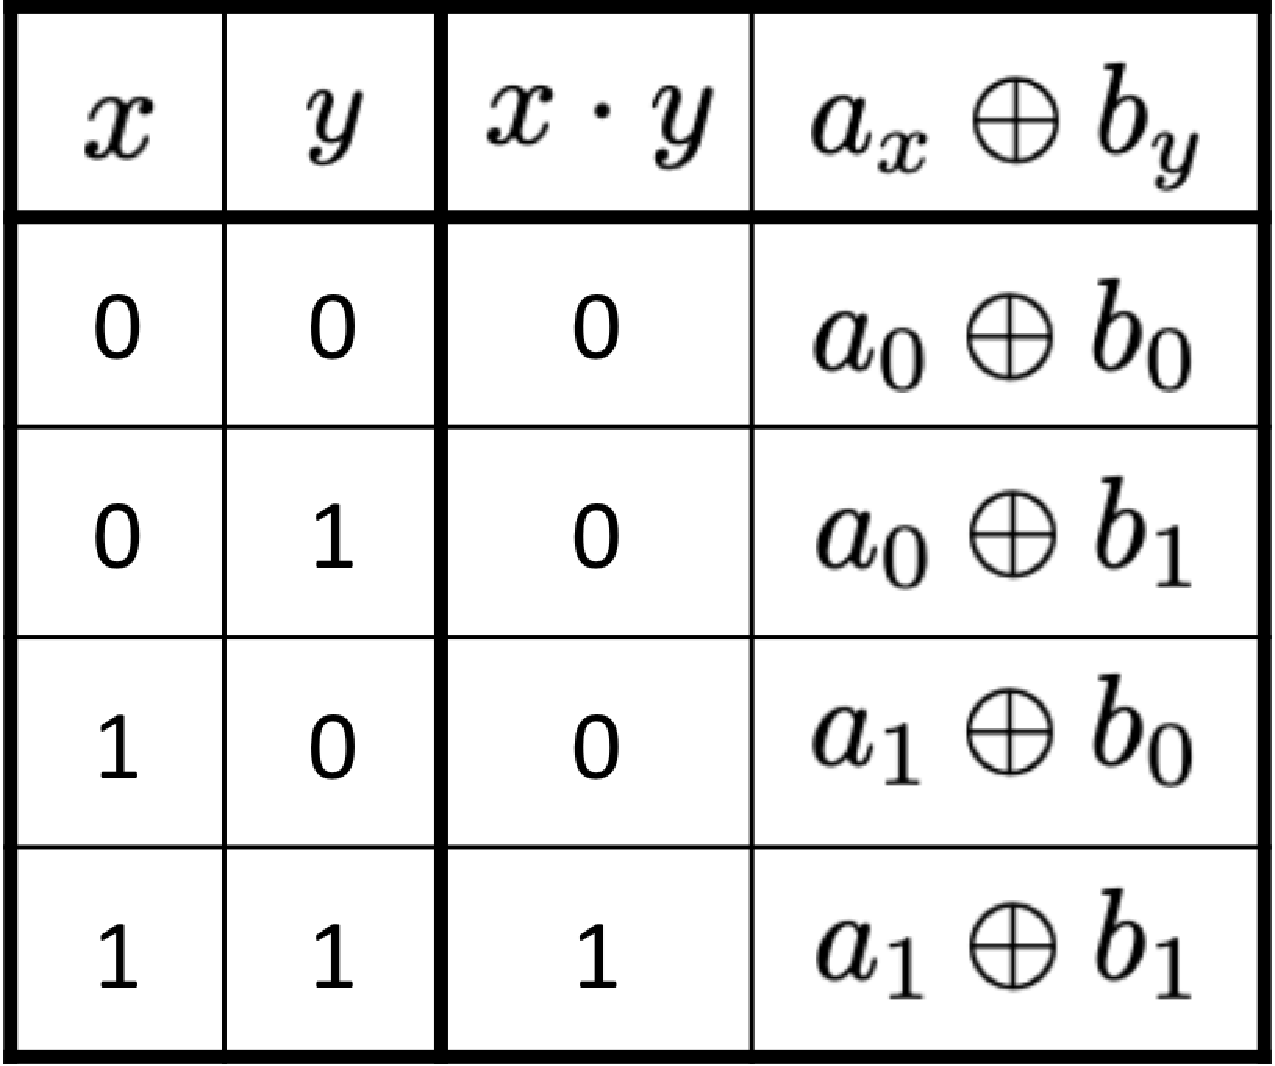
\includegraphics[width=0.8\textwidth]{lesson4/CHSH_table.pdf}
    \label{fig: 1}
    \begin{center}
        \caption{CHSHゲーム表}
    \end{center}
\end{figure}
表で見える通り、それはもちろん00, 01, 10, 11の4つの選択肢があるでしょ。そうすると$x y = 0$が3つのケースには0
なんですけれども一番下の行だけは1になる場合ですね。

じゃあ戦略として
は、もしAさんとBさんはそのxとy次第にはメッセージを決める場合にはまあそういうふうには$a_x$と$b_y$で書きましょう。そうすると100\%勝つ戦略は存在しない。まあこの場合だったら$x y$は3つのケースには0なんですが最後の係数だけには1になるでしょ。
その4つの選択肢なんですがじゃあどうやって決めるんでしょう。例えば
AさんとBさんは必ず0を返す場合にはa = b = 0の場合だったらまあいつ
も$a \oplus b = 0$なんでこの一番上の行には0 = 0、次は0 = 0、その次は0 = 0。最後の行だけは$1 \neq 0$ではないのでまあ3つのケースにはwinと一つのケースだけはloss
でしょ。3ケース勝ちで一つのケースだけ負けになるでしょ。こういう
戦略を使う場合には勝ちの確率は\textbf{75\%}なんですが、そうするとまあ
それがすごく簡単な戦略の例なんですけれども戦略はどれでも決める
場合には、どんな戦略でも勝てるならこの75\%より超える可能性はない
です:
% insert annotated table of possibilities
\begin{figure}[H]
    \centering
    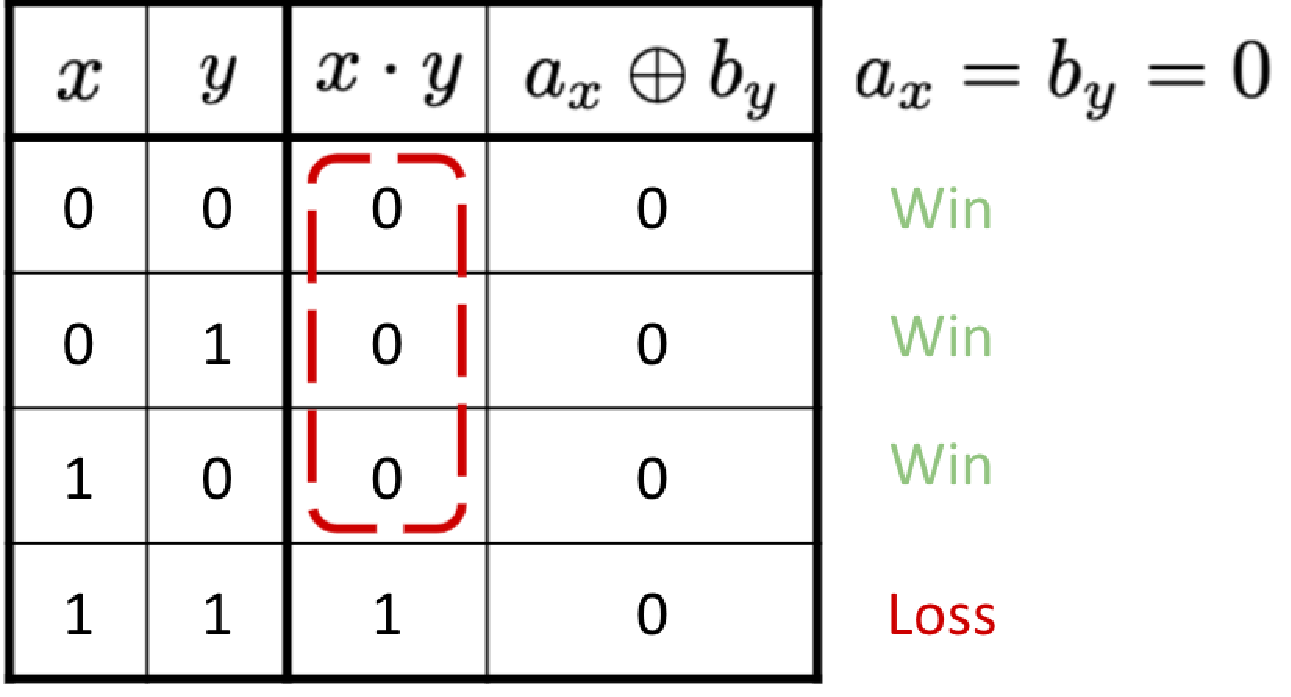
\includegraphics[width=0.8\textwidth]{lesson4/CHSH_annotated_table.pdf}
    \label{fig: 1}
    \begin{center}
        \caption{CHSHゲーム表+説明}
    \end{center}
\end{figure}
これがまあ証明はあるんです。けれども今回はちょっと証明は
おいといて量子の場合にも見てみましょう。

\subsection{量子戦略}
さて量子の場合だったらAさんとBさんもまだ古典のメッセージを交換するのは禁止なんですがまあさきにゲームが始まる前に\textbf{AさんとBさんは量子の状態をシェアする}ことを前提として見てみましょう:
% insert quantum diagram
\begin{figure}[H]
    \centering
    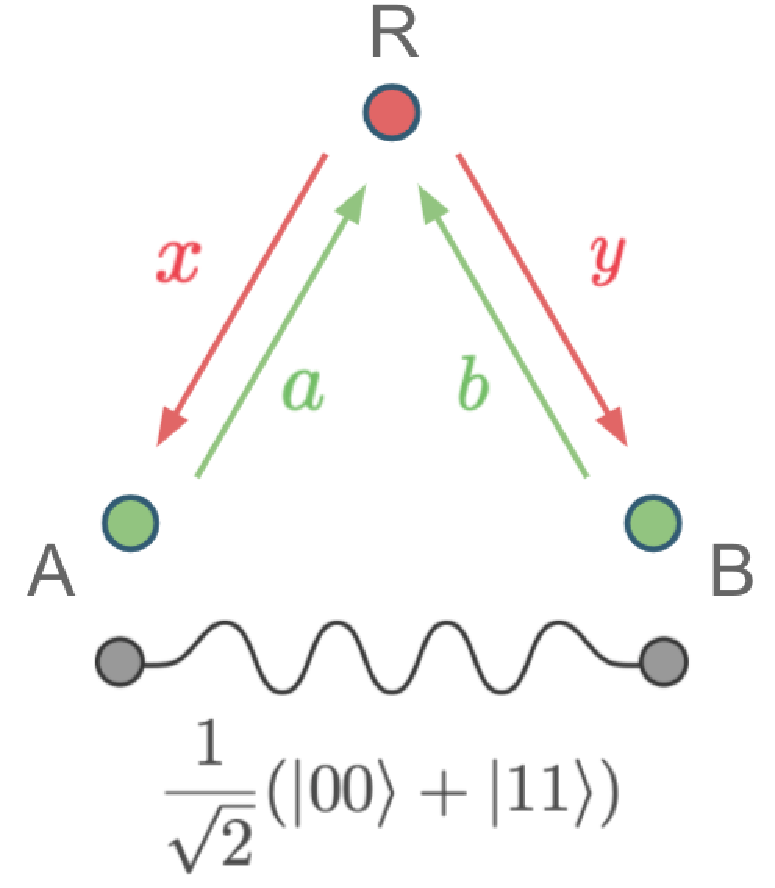
\includegraphics[width=0.5\textwidth]{lesson4/CHSH_quantum_diagram.pdf}
    \label{fig: 1}
    \begin{center}
        \caption{量子版}
    \end{center}
\end{figure}
2キュービットのステートなんですがAさんとBさんはひとつのキュービットずつ持つ場合にはこの状態が例えば
$\ket{00} + \ket{11}$の状態をシェアするとゲームはどういうふうに進むんでしょう?
これがこの\textbf{エンタングルメント}と言いますけれどもあと
でもうちょっと説明しますが。例えば、Aさんがこの戦略を立てます。
\begin{itemize}
    \item いただいたxのビットが$x=0$の場合だったら$Z$の基底で測定
します。
    \item $x = 1$の場合だったら$X$の基底で測定します。
\end{itemize}戦略
この前のステップで説明した測定の手法を使うんですがまあそうするとどうなる
でしょう。$a = 0$の場合にはそれがaのメッセージを0としてそれが
返事をすることはあの$+1$の結果が出てくる場合になる。例えばアウトカムの場合にその測定の結果は-1の場合だったら$a=1$のビット
を送ること。

Bの場合だったらこういう基底じゃなくて
斜めの基底まあ斜めっていうのはそれがそのbloch球使ってそれが
斜めと言えるんですけど例えば
\begin{itemize}
    \item $y=0$のビットだったら$\frac{1}{\sqrt{2}}(Z + X)$
の基底で測定すること。こういうふうも可能でしょ。この場合の測定
の説明にするとまあいろいろな手法にはいろんな基底で測定をする
ことは可能だと説明したと思います。
    \item じゃあ$y=1$の場合にはそれと直行な基底で$\frac{1}{\sqrt{2}}(Z-X)$のベーシスで測定する場合。
\end{itemize}
じゃあこういう戦略をさきに立てると結果はどうなるでしょう?

Bの戦略が$+1$の測定の結果が出てくると$b=0$。$-1$の結果が出てきたら$b = 1$のビットを送ります。そうするとAの返事するビットとBの返事するビットは小文字のaとbがこの量子状態の測定の結果次第には返事の小文字のaとbの
数字を決めます。そうすると勝ちの確率は75\%を超えて\textbf{85\%}にはなる。この場合だったらこれが +10\%にはなるんですよね。これが古典の場合
よりなにかできてるんでしょう。これが量子の状態のおかげで。
% Quantum まとめ guide
\begin{figure}[H]
    \centering
    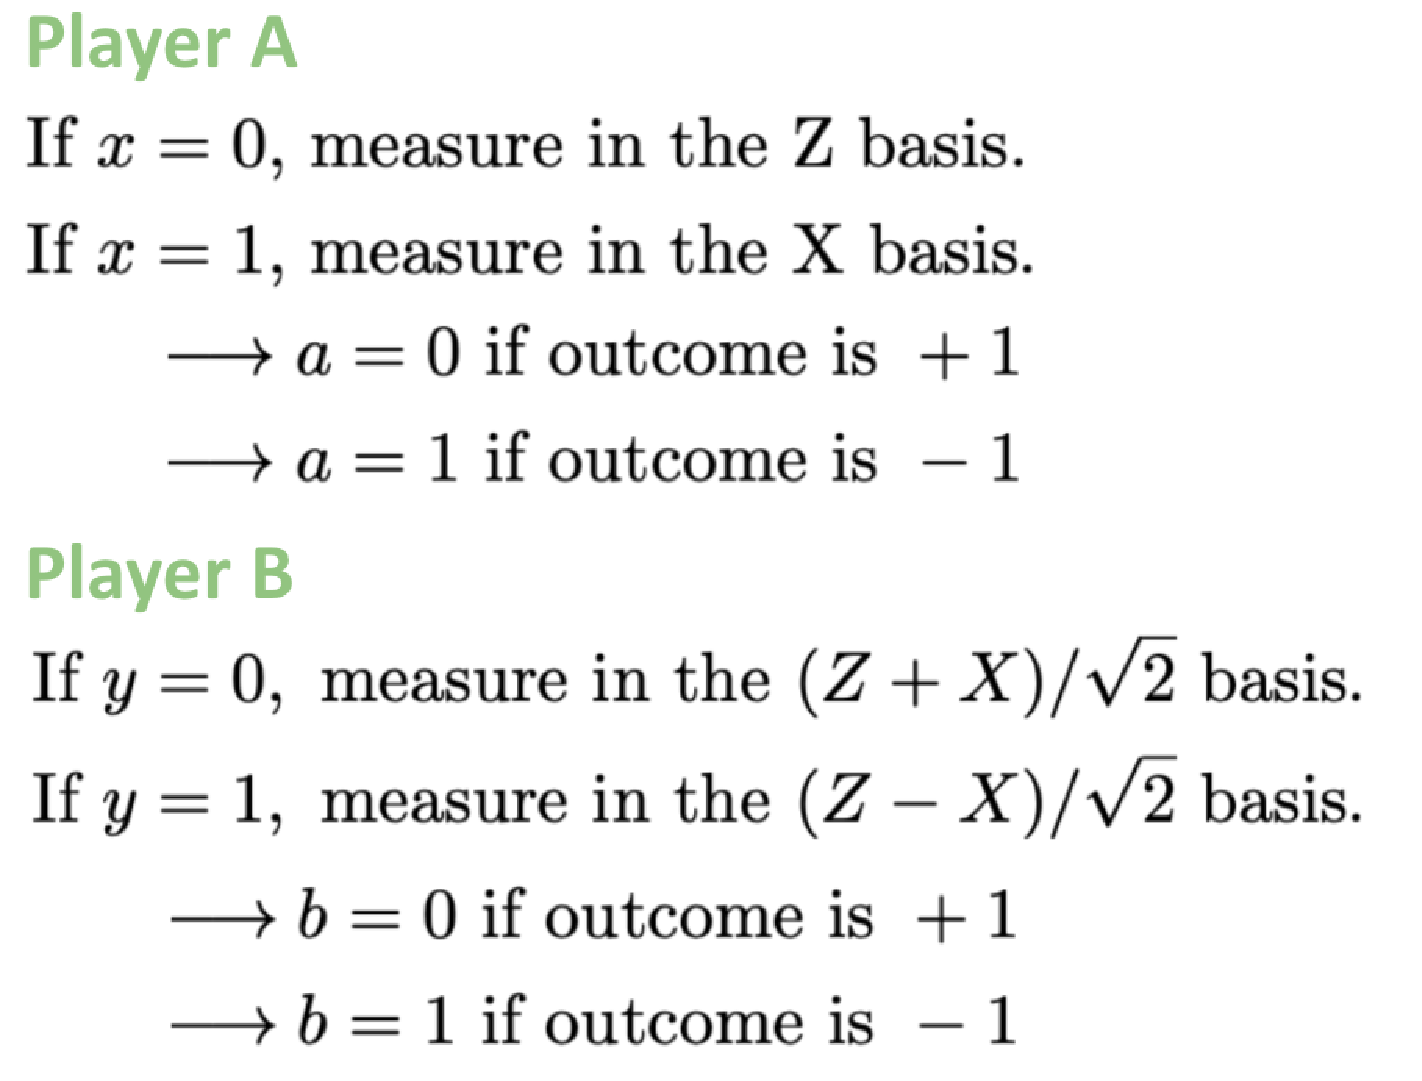
\includegraphics[width=0.8\textwidth]{lesson4/CHSH_quantum_guide.pdf}
    \label{fig: 1}
    \begin{center}
        \caption{量子版まとめ}
    \end{center}
\end{figure}


%%%%%%%%%%%%%%%%%%%%%%%%%%%%%%%%%%%%%%%%%%%
\section{量子もつれ}
2キュービットのステートをもうちょっと見てみましょう。
この前にはレッスン2のステップ5で説明したんですけれども
\textbf{tensor product}(テンソル積)について見てみましょう。
\subsection{Local -> Global 状態}
% insert intro slide
じゃあ例えば2つのキュービットがあって
キュービットAとキュービットBの場合にはどこのステートだったら
AとBは独立と言えるでしょう。独立にしているなら$\ket{\psi}_A = \ket{0}$の場合には$\ket{\psi}_B = \ket{0}$の場合にはAとBの関連はないのであまり関係ないでしょう。\textbf{global state}というのはこれを合わせて2つのキュービット複数のキュービットの状態を一つの数式で書けるとこの場合にはテンソル
積を使って$\ket{\psi}_A \otimes \ket{\psi}_B$にすると$\ket{00}$の状態
になるでしょ。

まあもう一つの例にすると:
% Insert 0-ket, +ket here
例えば$\ket{\psi}_A=0$の場合には$\ket{\psi}_B = \ket{+}$の場合だったら
そのグローバルステートには全体の状態をかけると$\ket{0}\ket{+}$になると
$\ket{00} + \ket{01}$ まあもちろんこれが正規化にするためには$\frac{1}{\sqrt2}$の係数をしなければならないんですけれどもこの場合には重要なポイントは、$\ket{0}$が左側にすると両タームの左側になって、$\ket{+}$の場合には右側には 0+1になるので全世界のa+bの状態を一つの数式にすると00 + 01になる。

\subsection{Global -> Local 状態}
さて他のステートには例えには独立の状態じゃなくて合わせてなにかの関係あるステートの場合にはどういうふうには各ステートには書くでしょう?
グローバルステートからlocalステートに分ける場合。

\begin{equation}
\ket{\psi}_{AB} = \frac{1}{\sqrt2}(\ket{00} + \ket{11})
\end{equation}
まあ例えば上の状態はさっきのステップで見たんですが$(\ket{00} + \ket{11})$の場合には0
と1の状態は独立ではない。AとBの状態は独立にはなってないでしょ
全体のステートが$(\ket{00} + \ket{11})$になると
まあ$\ket{\psi}_A$と$\ket{\psi}_B$は数学的にどうなるでしょう?

% Insert slide 
0に$\ket{\psi}_A$の場合はまあ1つのキュービットに書きたい場合にはいつも
使っている0と1の基底で$a_0\ket{0}+a_1\ket{1}$で$\ket{\psi}_B$の場合は$b_0\ket{0}+b_1\ket{1}$でこれはもちろん正規化の状態にはしなければならない。
のでまあ$a_0$と$a_1$がそれが合わせて正規化しなければならないし$b_0$と$b_1$は一緒。ですが全体のステートがこの場合には$(\ket{00} +\ket{11})$の場合にはどういうふうには数学的にはAとBに分けるでしょう。
まあこの場合にはAは$a_0\ket{0}+a_1\ket{1}$とBは
は$b_0\ket{0}$+$b_1\ket{1}$ならこれのテンソル積にするとどうなるんでしょう:
\begin{equation}
|\psi\rangle_{A} \otimes|\psi\rangle_{B}=\left(a_{0}|0\rangle+a_{1}|1\rangle\right) \otimes\left(b_{0}|0\rangle+b_{1}|1\rangle\right)
\end{equation}
\iffalse
まあこの4つのタームが入っている

0:04:09.620,0:04:21.940
と数式になるんですがこれが$a_0$
かける$b_0$の00+$a_0$$b_1$の01+$a_1$$b_0$の10+$a_1$$b_1$

0:04:21.940,0:04:34.930
の11にはなるんでしょそう
\fi

するとまあこの$a_0b_0$は\textbf{式4.1}の$\ket{\psi}_{AB}$の$\ket{00}$と合わせなければならないし、$a_1b_1$は\textbf{式4.1}の$\ket{\psi}_{AB}$の$\ket{11}$の状態に合わせなければならない。そうすると:
\begin{equation}
a_{0} b_{0}=a_{1} b_{1}=\frac{1}{\sqrt{2}}
\end{equation}
まあまあこれがかんたんな代数なんですが、問題はそうすると$a_0b_1$と$a_1b_0$が0しなければならない。この$a_0b_1$は、\textbf{式4.1}のところにはその状態にはそういうタームはないし、$a_1b_0$のタームはないので、これが不可能にはなるでしょ:
\begin{equation}
a_{0} b_{1}=a_{1} b_{0}=0 \quad \longrightarrow a_{0}=0 \quad \text { or } \quad b_{1}=0
\end{equation}
この場合だったら、$a_0=0$か$b_1=0$が\textbf{式3.3}のところに決まっているのでそれが不可能になるんです。

さてていうことは、\textbf{すべての可能なグローバルな状態がテンソル積には書けるわけではない。}そういうふうにするとグローバルステートがあるんですけれども各キュービットの
正式的なローカルステートにはならない。
\subsection{Product State と Entangled State}
まあもうちょっと見てみるとそのさっきのproduct stateには正規状態なんですが\textbf{正規状態だったら必ずAとBは分けられる。}そうすると$\ket{\psi}_{AB} = \ket{\psi}_A \otimes \ket{\psi}_B$は可能。

そうするとこれがaだけを持って
いればAの状態がローカルステートの状態だけには完全の情報を持っているんですけれどもBの状態だったらBについての情報を完全に持っているんでAとBは各キュービットについている情報を持っていればグローバルステートの全体としてはその情報を持ちます。

\textbf{Entangled states}(量子もつれの状態)にはそのグローバルステートそういうふうにはなりません。AとBがある場合なんですが$\ket{\psi}_{AB}= \ket{\psi}_A\ket{\psi}_B$にはなりません:
\begin{equation}
|\psi\rangle_{A B} \neq|\psi\rangle_{A} \otimes|\psi\rangle_{B}
\end{equation}
これはノットイコールの状態になります。というわけは完璧な情報を持ち
たいなら全体のシステムにAとBあわせての状態の情報を知らないとその情報を持ってなければならないんですけれども独立にはならないから一緒の状態になってますから。


\section{ベル状態}
この前には2キュービットのステート
は話ししたんですけれども量子もつれについてはどうなるのか
じゃあもうちょっと具体的な例を見てみましょう。重要なステート
の種類は\textbf{ベルステート}といいます。4つのベルステートがあるんです
けれども基本的にparityとしては2つのキュービットはAとBはイコール
になってるか位相は0かパイになるか4つのケースにわけて4つのベル
状態になります。
\begin{equation}
\begin{aligned}
\ket{\Phi^{+}}&=\frac{1}{\sqrt{2}}(|00\rangle+|11\rangle) &\left|\Phi^{-}\right\rangle=\frac{1}{\sqrt{2}}(|00\rangle-|11\rangle) \\
\ket{\Psi^{+}}&=\frac{1}{\sqrt{2}}(|01\rangle+|10\rangle) &\left|\Psi^{-}\right\rangle=\frac{1}{\sqrt{2}}(|01\rangle-|10\rangle)
\end{aligned}
\end{equation}
今まで見たのは$\ket{00}+\ket{11}$なんですがこれが$\Phi^{+}$のベル
ステートと言います。するんですけれども位相だけは変更すると
$\ket{00}-\ket{11}$になってこれが$\Phi^{-}$のステートになります。ですがこれが左側のキュービットと右側のキュービットの状態は一緒なんですけれども、
0か1か、異なる場合もあるんです。$\ket{01}+\ket{10}$の場合これは$\Psi^{+}$の状態と言いますけれどもこれも位相変換にすると$\ket{01}-\ket{10}$にするとこれが$\Psi^{-}$の状態と言います。この4つのステートは\textbf{ベルステート}と言います。これはいろんな使う手法があるんです:
\begin{itemize}
    \item 量子コミュニケーション
    \item 量子コンピューテーション
    \item 量子計算
    \item 量子鍵配送
    
\end{itemize}


%%%%%%%%%%%%%%%%%%%%%%%%%%%%%%%%%%%%%%%%%%%%%%%
\subsection{ベル基底}
さっきの言ってた例がちょっと複雑に見えるんですがこれが\textbf{computational basis}(計算基底)との言い方なんですがbell basisがこういうふうにも書き直せること:
\begin{equation}
\begin{aligned}
|00\rangle &=\frac{1}{\sqrt{2}}\left(\left|\Phi^{+}\right\rangle+\left|\Phi^{-}\right\rangle\right) & 
\ket{01} = \frac{1}{\sqrt2}(\ket{\Psi^{+}} - \ket{\Psi^{-}}) \\
|10\rangle &=\frac{1}{\sqrt{2}}\left(\left|\Psi^{+}\right\rangle-\left|\Psi^{-}\right\rangle\right) & 
\ket{11} = \frac{1}{\sqrt2}(\ket{\Phi^{+}} - \ket{\Phi^{-}})
\end{aligned}
\end{equation}

でまあもちろん計算基底としては4つの候補があるんですが、$\ket{00}$,$\ket{01}$,$\ket{10}$, $\ket{11}$,$\ket{00}$の状態が\textbf{式1.7}で表されているようにベルステートで書き換えられます。
\iffalse
だったら:
phi+ + phi- /  +  - psi-これが位相には
さっきのところと違うんですが

0:02:59.190,0:03:07.200
で11の場合だったらphi+ - phi-にする
とまあこういうふうには4つのbell

0:03:07.200,0:03:14.810
basisをつかって4つのベル状態を
使って4つの計算基底を使って書き

0:03:14.810,0:03:22.049
直せることです。
\fi
そうするとまあ
もうちょっと汎用的な2キュービットのステートにすると:
\begin{equation}
|\psi\rangle=\alpha|00\rangle+\beta|01\rangle+\gamma|10\rangle+\delta|11\rangle
\end{equation}
すると\textbf{式4.7}を用いて\textbf{式4.8}を書き換えると:
\begin{equation}
|\psi\rangle=\frac{\alpha+\beta}{\sqrt{2}}\left|\Phi^{+}\right\rangle+\frac{\alpha-\beta}{\sqrt{2}}\left|\Phi^{-}\right\rangle+\frac{\gamma+\delta}{\sqrt{2}}\left|\Psi^{+}\right\rangle+\frac{\gamma-\delta}{\sqrt{2}}\left|\Psi^{-}\right\rangle
\end{equation}
\iffalse
00はphi+ + phi-にするとまあちょっと

0:03:47.049,0:03:59.010
代数やってみると最初の方はphi
+の状態がalpha + beta / √2  - の状態は

0:03:59.010,0:04:07.599
alpha - betaになってpsi+はgamma+delta
になってpsi-はgamma - deltaにはすること

0:04:07.599,0:04:13.370
になるでしょ。
\fi
ていうわけはこの汎用的な2キュービットステートは計算基底も書けるしベルの状態を使って基底としては基底セットとして使ってそれも書き直せるんです。
\subsection{ベル基底測定}
もう一つの使い方があるんですがベル基底としてはそれが測定も可能です:
\begin{equation}
|\psi\rangle=\frac{\alpha+\beta}{\sqrt{2}}\left|\Phi^{+}\right\rangle+\frac{\alpha-\beta}{\sqrt{2}}\left|\Phi^{-}\right\rangle+\frac{\gamma+\delta}{\sqrt{2}}\left|\Psi^{+}\right\rangle+\frac{\gamma-\delta}{\sqrt{2}}\left|\Psi^{-}\right\rangle
\end{equation}

まあ例えば上の状態はさっきのスライドの状態がこれ4つのタームが入っているんですがそれが確率的にはいつもの使っている絶対値を使って:
\begin{equation}
\begin{aligned}
&\operatorname{Prob}\left\{\left|\Phi^{+}\right\rangle\right\}=\frac{|\alpha+\beta|^{2}}{2} \quad \operatorname{Prob}\left\{\left|\Phi^{-}\right\rangle\right\}=\frac{|\alpha-\beta|^{2}}{2} \\
&\operatorname{Prob}\left\{\left|\Psi^{+}\right\rangle\right\}=\frac{|\gamma+\delta|^{2}}{2} \quad \operatorname{Prob}\left\{\left|\Psi^{-}\right\rangle\right\}=\frac{|\gamma-\delta|^{2}}{2}
\end{aligned}
\end{equation}
\iffalse
alpha + beta
絶対値の事情わる2がそれがphi+

0:04:55.170,0:05:03.290
の確率にはなるでしょ。まあ算数
繰り返すとこれが4つの状態に同じ

0:05:03.290,0:05:06.190
ふうになるんでしょ
\fi

でこのベル測定がいろんな通信
のプロトコルに使ってるんです。とくに\textbf{量子状態のテレポーテーション}
と\textbf{エンタングルメントスワッピング}という手法なんですがそれがアルゴリズムなんでそれが今後のレッスンに説明します。
\subsection{ベル状態のLocal測定 }
でローカルの場合にちょっと見てみましょう。ひとつのキュービット
だけを測定するとそれは\textbf{ローカルメジャーメント}といってそれが1つのキュービットだけの状態の情報にはなるんですが例えば下のベルステート使いましょう:
\begin{equation}
\left|\Phi^{+}\right\rangle=\frac{1}{\sqrt{2}}(|00\rangle+|11\rangle)
\end{equation}
$\ket{phi^{+}}= \frac{1}{\sqrt{2}}(\ket{00}+\ket{11})$なんで左側のキュービットか右側のキュービットだけを独立に測定すると、例えば\textit{Xの基底}で測定
すると$+1$の出てくる確率と$-1$の出てくる
確率は2つとも50\%になります。Zの基底とYの基底に測定するとそれが全く一緒:
% add all bases having same outcome probabilities
\begin{figure}[H]
    \centering
    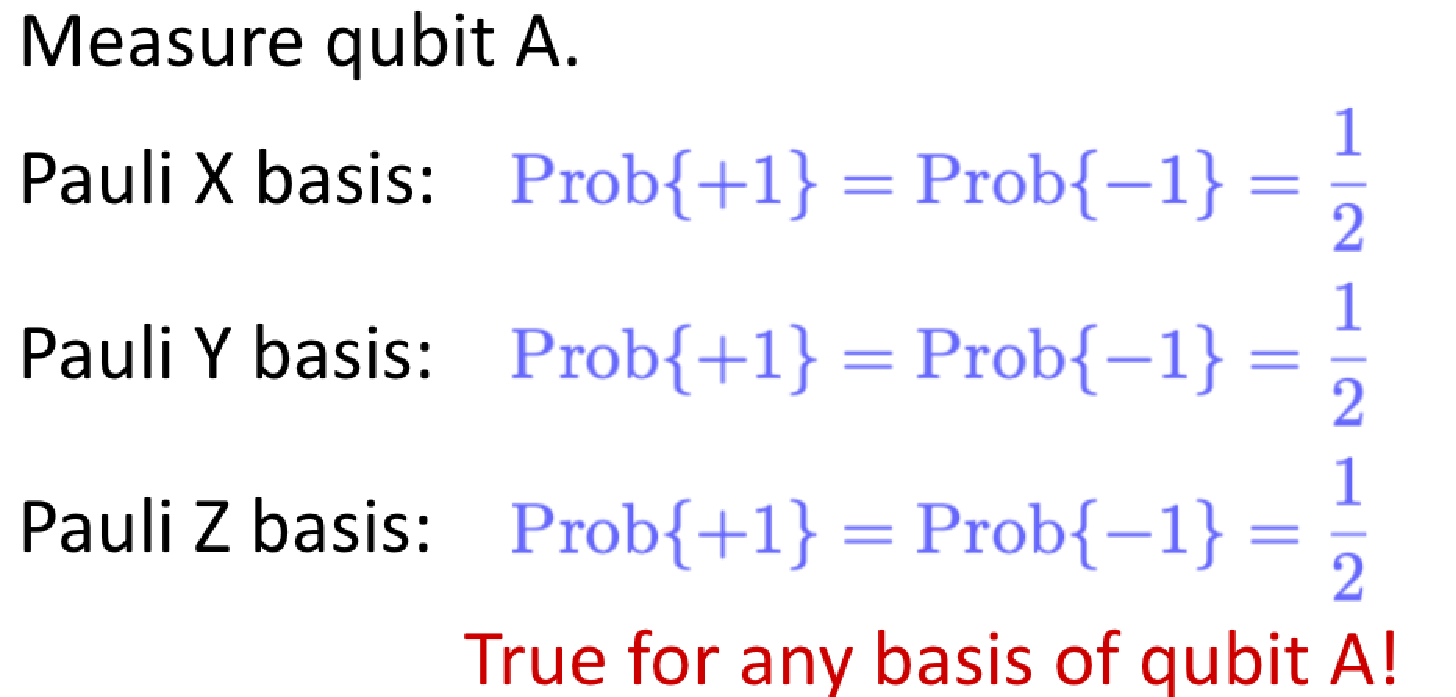
\includegraphics[width=0.8\textwidth]{lesson4/Qubit_A.pdf}
    \label{fig: 1}
    \begin{center}
        \caption{Aの測定結果}
    \end{center}
\end{figure}
%状態とyの状態

+1の状態か-1の状態の測定の結果になることは全ては50\%になります。つまりAの測定の基底としてはなんでもの基底を使えば+1と-1が出てくる確率は全ては50-50なんです。

するとB側を見てみると全く一緒なんですが各状態については出てくる測定の結果
がそれの確率が50\%です:
% B Qubit measurement results
\begin{figure}[H]
    \centering
    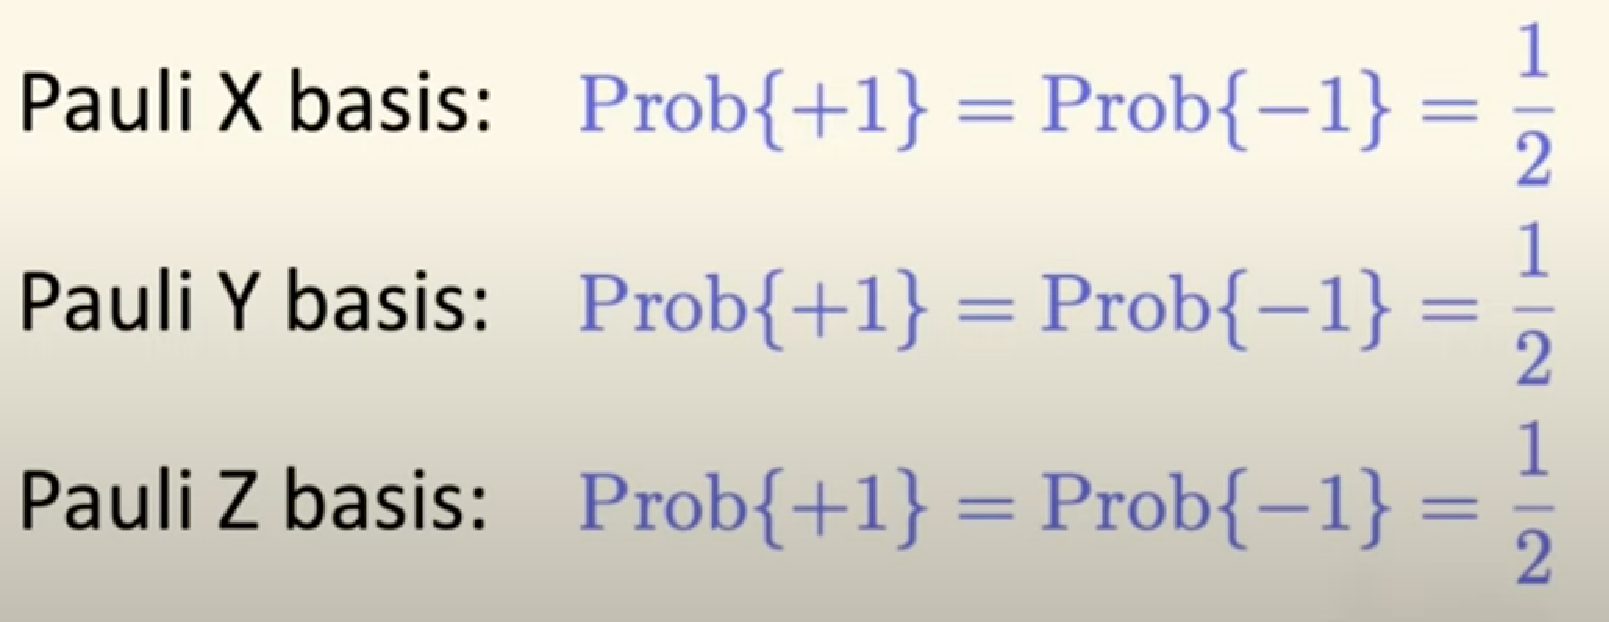
\includegraphics[width=0.8\textwidth]{lesson4/Qubit_B.pdf}
    \label{fig: 1}
    \begin{center}
        \caption{Bの測定結果}
    \end{center}
\end{figure}
これもBの基底には測定の基底に問わずにそういう状態になるでしょ。つまり結果が完全にランダム。つまり情報は持ってません。その状態については何も知識はない。一つだけAのキュービットを持っているかBのキュービットを持っているか。それがインフォーメーションにはなりません。情報にはなりません。

つまり密度行列で書き直すと各キュービットの密度行列が:
\begin{equation}
\begin{aligned}
\rho_{A} &=\frac{1}{2}(|0\rangle\langle 0|+| 1\rangle\langle 1|) \\
\rho_{B} &=\frac{1}{2}(|0\rangle\langle 0|+| 1\rangle\langle 1|)
\end{aligned}
\end{equation}
$\ket{0}\bra{0}+\ket{1}\bra{1}$の2分の1にはなるでしょ。
このキュービット合わせて独立ではないんですけれどもこのキュービット合わせてグローバルステートにはfull状態にはなるんですが各キュービットについてはローカルの情報がないんですね。Aのキュービットは$\rho_{A}$と書き、bは$\rho_{b}$と書けます。けれどもAだけ持ってれば情報にはならないし、Bだけ持ってれば情報にはならないし。けれども一緒に2つとも持っているとその状態が
完全の状態にはなっててそれが情報が完璧になります。
\begin{figure}[H]
    \centering
    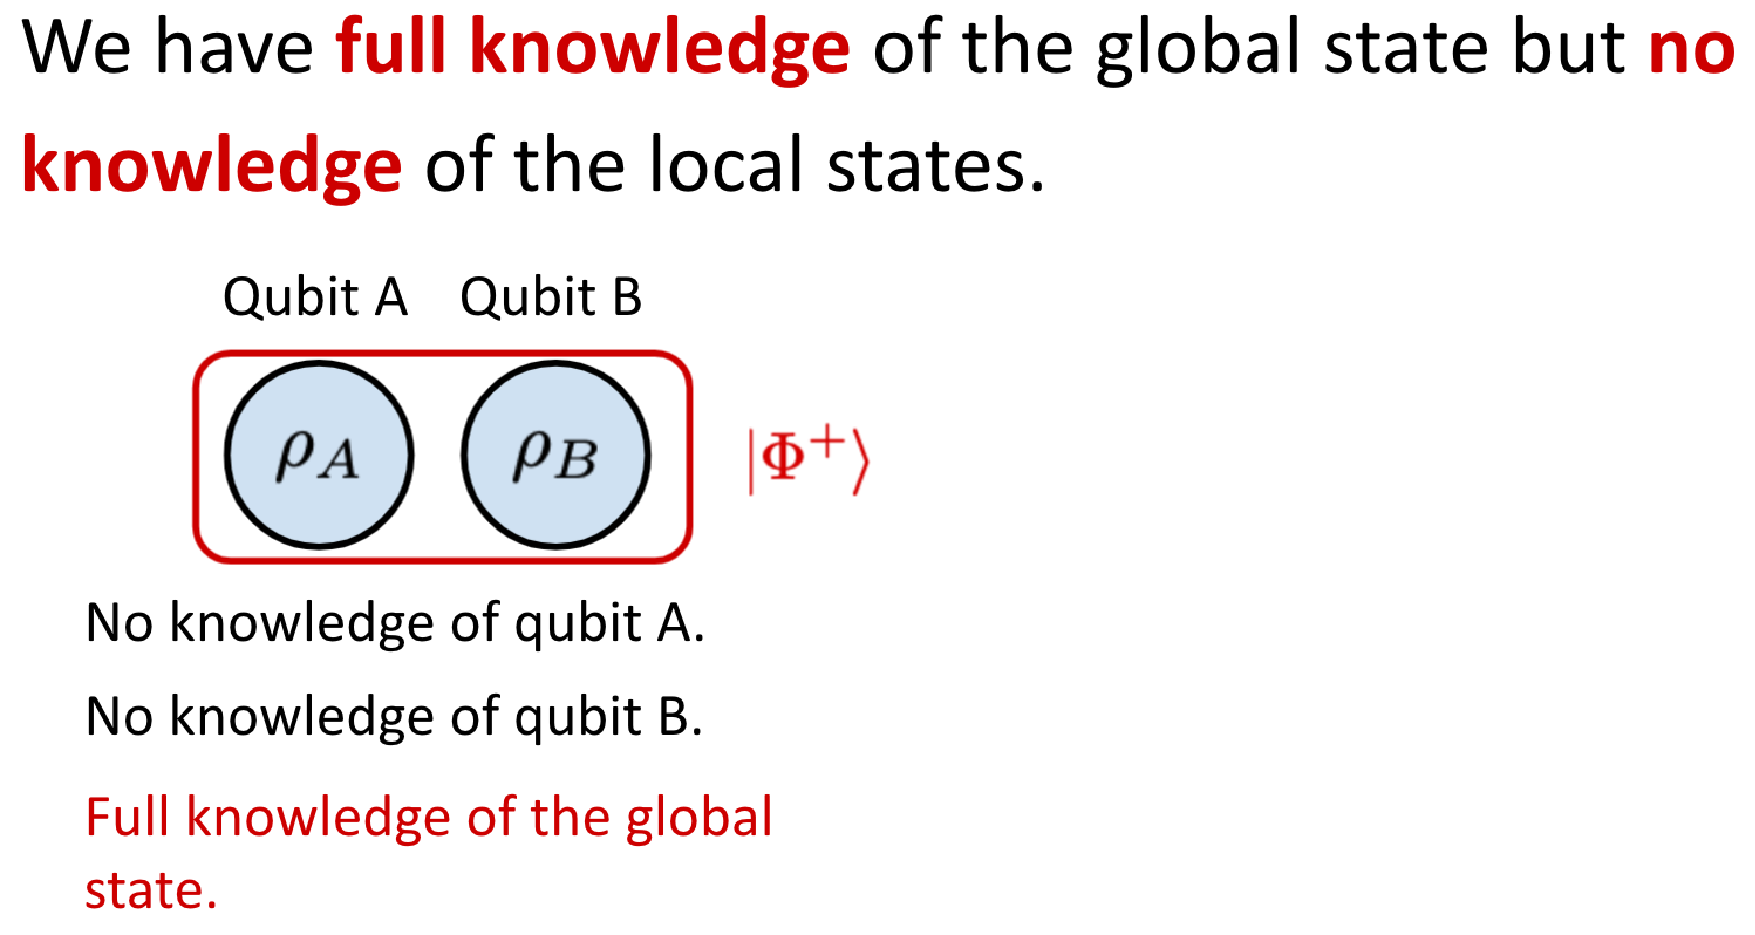
\includegraphics[width=1.0\textwidth]{lesson4/4.3_Recap.pdf}
    \label{fig: 1}
    \begin{center}
        \caption{ステップのまとめ}
    \end{center}
\end{figure}


%%%%%%%%%%%%%%%%%%%%%%%%%%%%%%%%%%%%%%%%%%%%%%%%%%%%%%
\section{SPDC (自発的パラメトリック下方変換)}
SPDC:つまり「自発的パラメトリック
下方変換」。英語ではSpontaneous Parametric Down-
Conversionと言いますけれども、これは特別な物理的な手法なんで\textbf{これが量子もつれを作ることです。}
% pic
\begin{figure}[H]
    \centering
    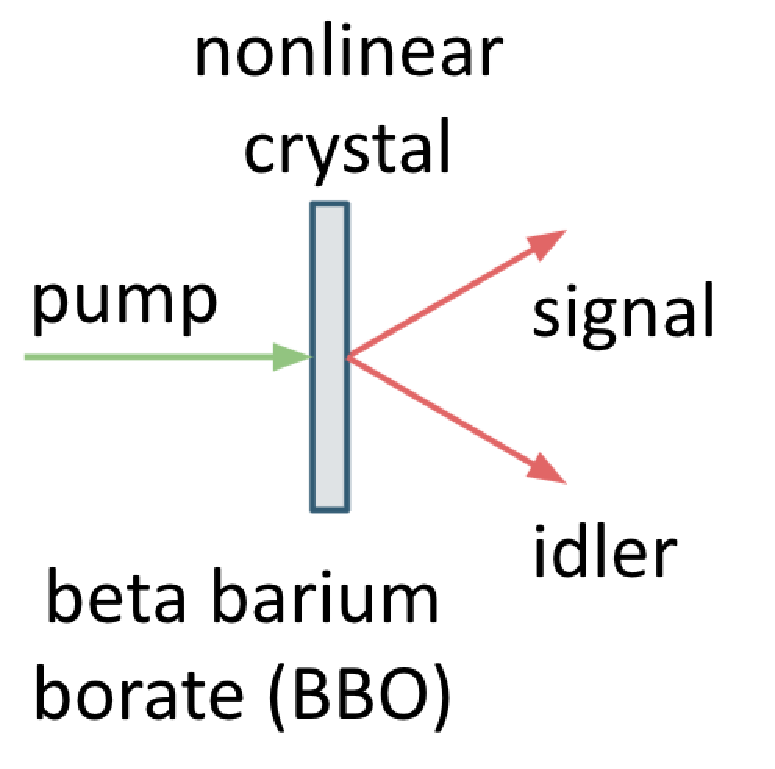
\includegraphics[width=0.8\textwidth]{lesson4/pump.pdf}
    \label{fig: 1}
    \begin{center}
        \caption{SPDC図}
    \end{center}
\end{figure}
上の画像は光子を使って、量子もつれの状態になっている二つの光子を作る手法です。この場合だったら1つの光子はインプットして2つの
光子がアウトプットになるんです。そのインプットの状態は緑の
矢印とアウトプットは赤い矢印。インプットの状態は\textbf{パンプ}(pump)
といいます。強いレーザーの光を入れるんでアウトプットが出てくる
のは2つの赤い光子が出てきます。それが\textbf{シグナル}と\textbf{アイドラー}と言います。これが非線形型のクリスタル水晶を通るんですけれどもその
種類が例えば\textbf{BBO}クリスタルと言いますけれどもBeta Barium Borateというものなんですがまあ他の種類もあるんですけれどもとりあえず
これが例として。でそのパンプの光が下の図のように水晶を通るんです:
\begin{figure}[H]
    \centering
    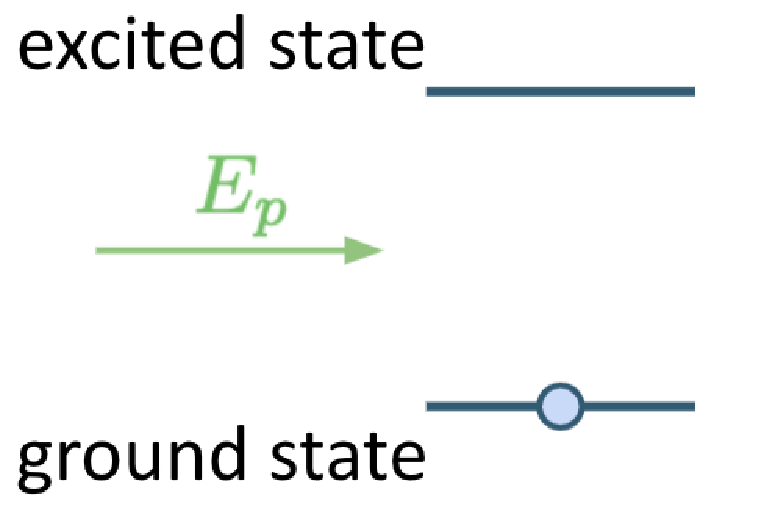
\includegraphics[width=0.5\textwidth]{lesson4/state1.pdf}
    \label{fig: 1}
    \begin{center}
        \caption{基底状態}
    \end{center}
\end{figure}
けれどもクリスタルに通してある原子がグラウンドステート(基底状態)のところからエキサイテッドステート(励起状態)には上がってくるんですけれども\textbf{Figure 4.11}だったら水平線はエネルギーレベルと言いますがそのエネルギー
が下のグラウンドステートからエキサイテッドステートにはなって、降りてくるときはもとのエネルギーレベルには戻る場合は結構あるんです:
\begin{figure}[H]
  \centering
  \begin{minipage}[b]{0.3\textwidth}
    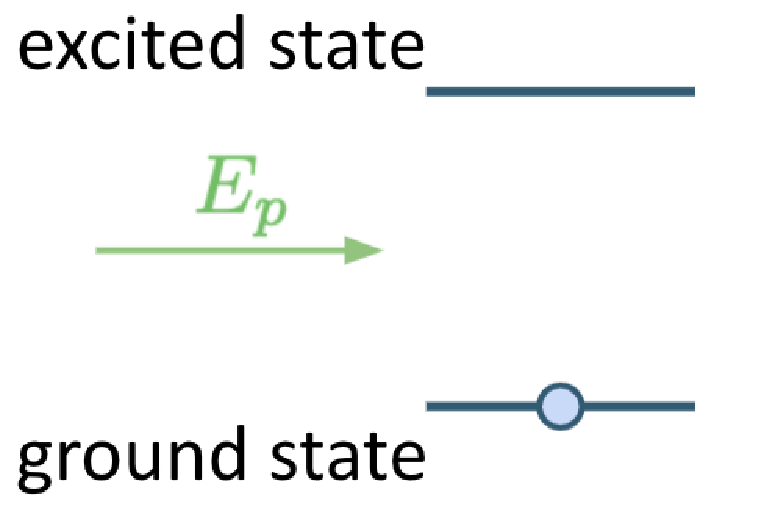
\includegraphics[width=\textwidth]{lesson4/state1.pdf}
    \caption{基底状態[状態1]}
  \end{minipage}
  \hfill
  \begin{minipage}[b]{0.3\textwidth}
    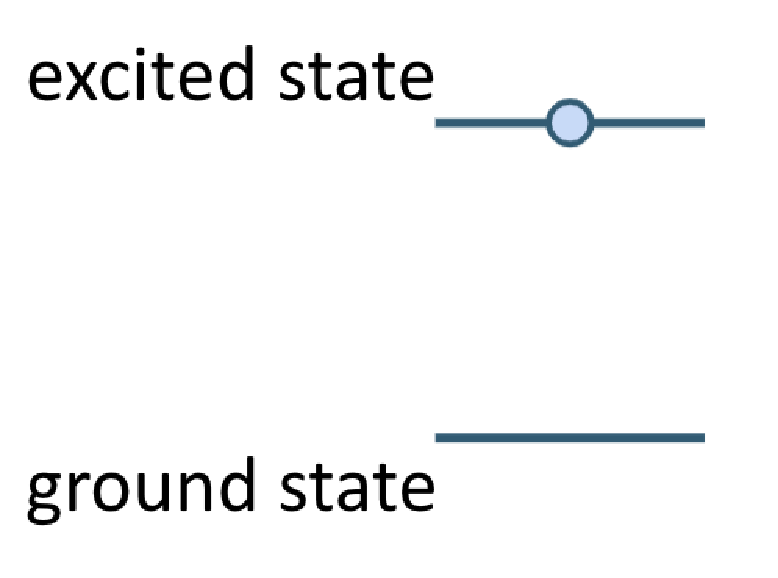
\includegraphics[width=\textwidth]{lesson4/state2.pdf}
    \caption{励起状態[状態2]}
  \end{minipage}
  \hfill
  \begin{minipage}[b]{0.3\textwidth}
    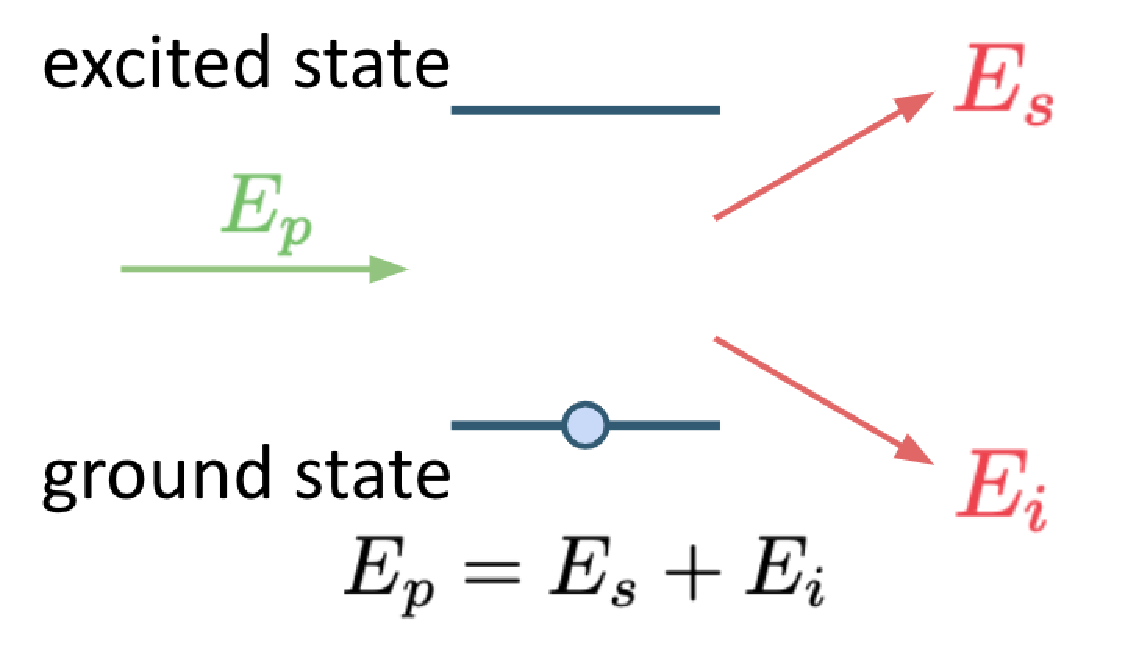
\includegraphics[width=\textwidth]{lesson4/state3.pdf}
    \caption{基底状態[状態3]}
  \end{minipage}
\end{figure}
\iffalse
\begin{figure}[H]
    \centering
    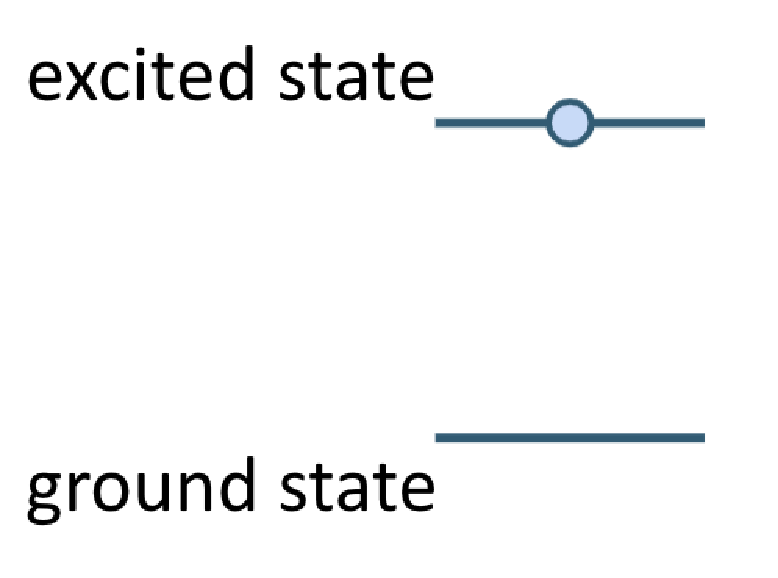
\includegraphics[width=0.5\textwidth]{lesson4/state2.pdf}
    \label{fig: 1}
    \begin{center}
        \caption{励起状態}
    \end{center}
\end{figure}
\begin{figure}[H]
    \centering
    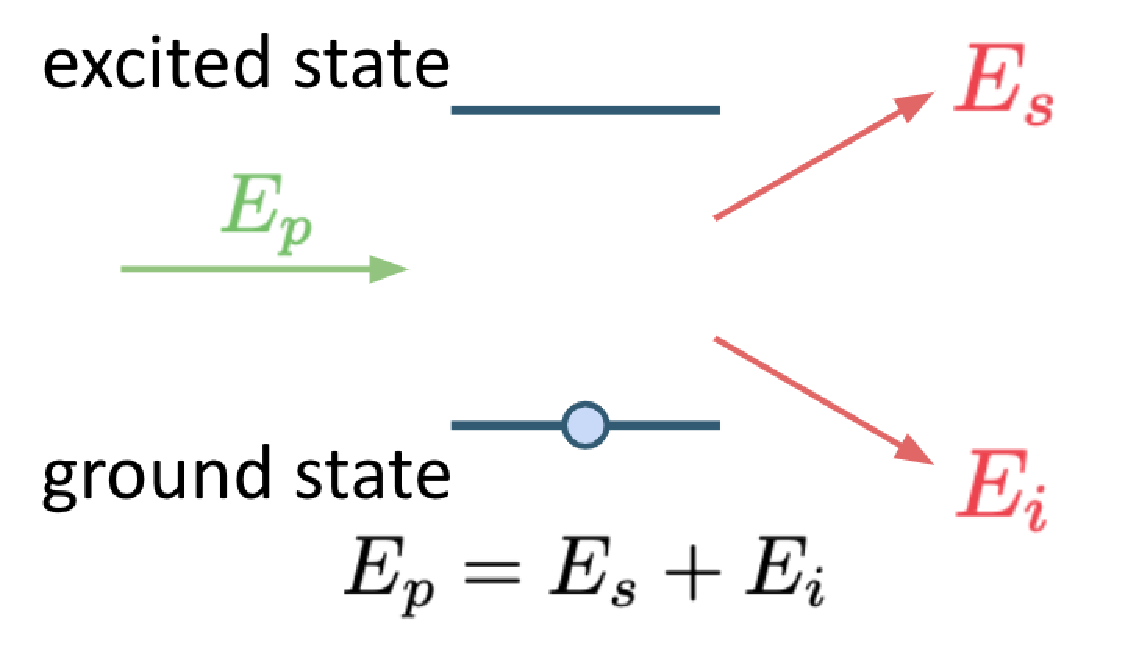
\includegraphics[width=0.5\textwidth]{lesson4/state3.pdf}
    \label{fig: 1}
    \begin{center}
        \caption{基底状態2}
    \end{center}
\end{figure}
\fi
それが出てくる場合には1つの光子か2つの光子にはなるですがインプットのエネルギーとアウトプットのエネルギーは一緒にしなければならないの$E_p = E_s + E_i$。
\subsection{偏光}
さてこれがどうやって使うことが
できるんでしょう。光子の偏光は勉強したことあると思うんですがこれがキュービットで表示しましょう:
\begin{figure}[H]
    \centering
    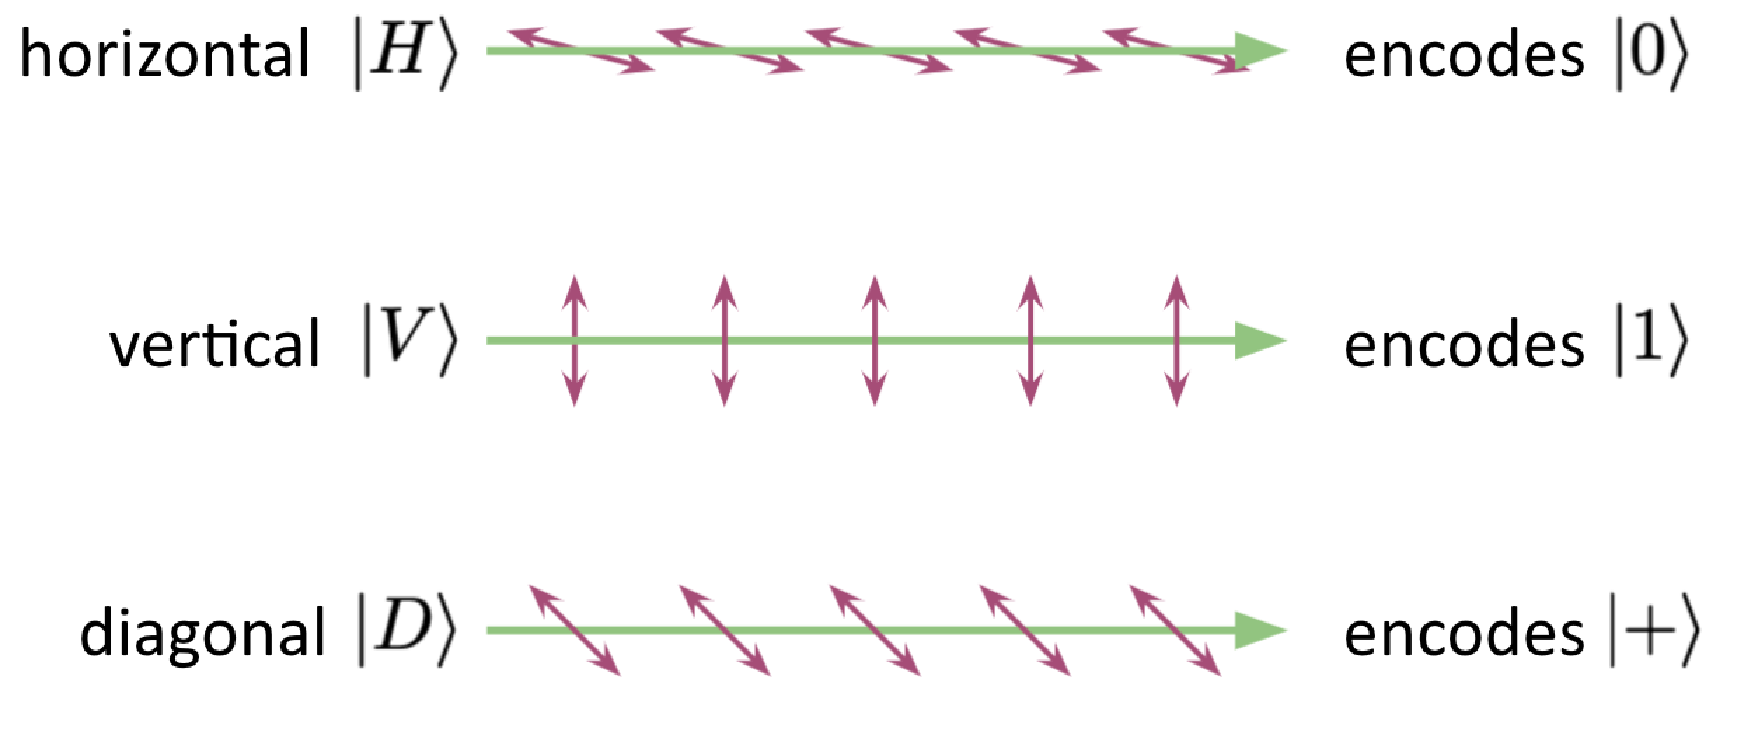
\includegraphics[width=0.8\textwidth]{lesson4/linear_polarization.pdf}
    \label{fig: 1}
    \begin{center}
        \caption{水平偏光・垂直偏光・対角偏光}
    \end{center}
\end{figure}
例えば水平の偏光これがhorizontalの状態を使うとこれを$\ket{0}$の状態と表示していて縦の偏光だったらこれが垂直の偏光なんですがこれが$\ket{1}$の状態を表示することにしましょう。そうすると斜めの場合には対角なんですがそれがダイアグナルと言いましてこれが$\ket{+}$の状態になる。これが対角になっているので\textit{半分水平と半分垂直}になっているんでしょさてこういう偏光を持っている。

光子がBBOクリスタルを通してどういう効果になるでしょう。まあそれはクリスタルの\textbf{optical axis}(光軸)によって変換は変わるんですけれども
% 14:30 Aug 21 ここまで
これが水平の場合(図4.15)だったら水平の偏光の光子を入れると変換して出てくる2つのキュービットが2つの光子が垂直の光子になるんです:
\begin{figure}[H]
    \centering
    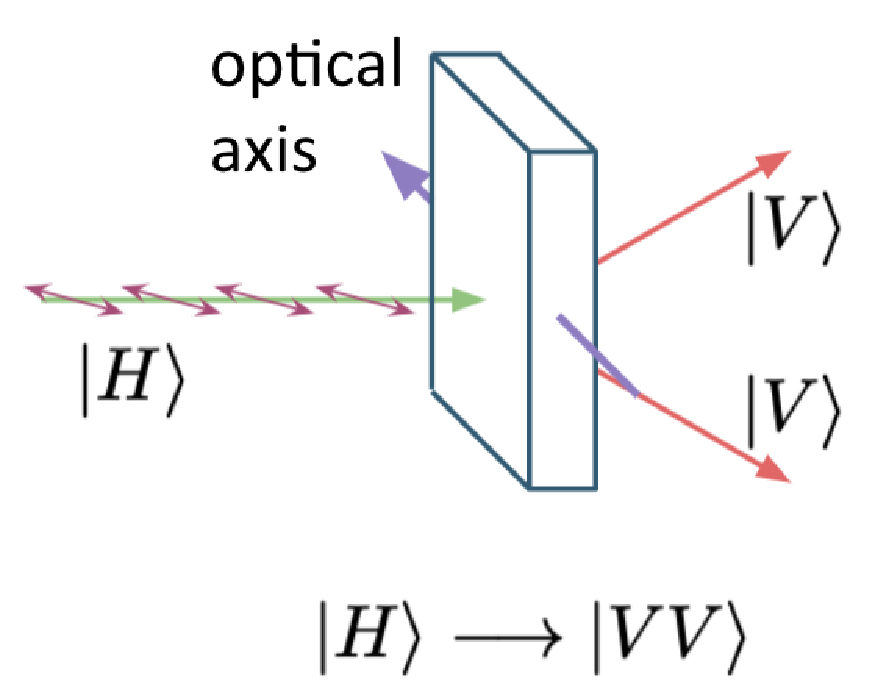
\includegraphics[width=0.8\textwidth]{lesson4/horizontal_optical_axis.pdf}
    \label{fig: 1}
    \begin{center}
        \caption{水平偏光}
    \end{center}
\end{figure}
インプットが水平偏光($\ket{H}$ならば、アウトプットの二つの光子は垂直偏光$\ket{V}$になるんです。

逆の方にすると、垂直の場合にはインプットの状態も垂直の偏光だったらアウトプットが水平偏光にはなるんでインプットが$\ket{V}$でアウトプットが$\ket{H}\ket{H}$なのでこれも
逆の方になるでしょ:
\begin{figure}[H]
   \centering
    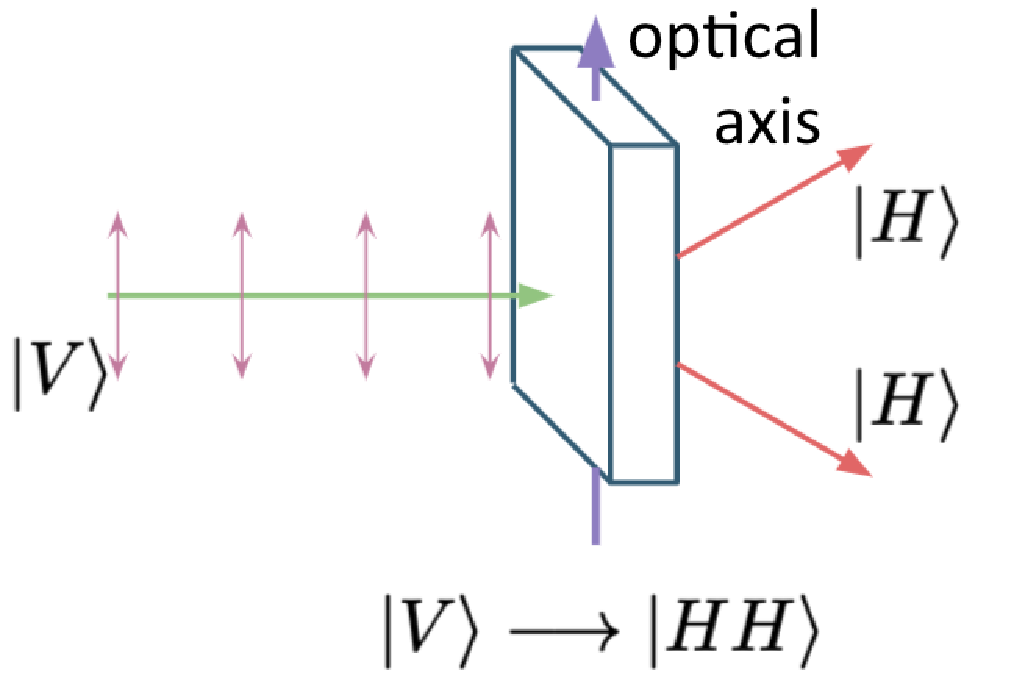
\includegraphics[width=0.8\textwidth]{lesson4/vertical_optical_axis.pdf}
    \label{fig: 1}
    \begin{center}
        \caption{垂直偏光}
    \end{center}
\end{figure}

\textit{必ずインプットのpolarizationとアウトプットのpolarizationは逆のことになります}。

\subsection{量子もつれ光子の生成}
さてこれがどうやって使って量子
もつれを作れるんでしょう。もつれを持っている光子になるんでしょう。
2つのクリスタルを使うんです。1つだけじゃなくて2つ合わせて。1つ
は縦と1つは横で水平と垂直なんです。対角光子を入れて時々光子
が前のクリスタルに変換になる場合または後ろのクリスタルに変換
になる場合には出てくる状態が$\frac{\ket{HH}+\ket{VV}}{\sqrt{2}}$にはなるんです。
量子もつれ生成過程が成功するのには、いくつかの条件があるんです:
\begin{enumerate}
    \item クリスタルはすごく薄くしなければならないんです。そうすると前の方に変換になったか後ろの方に変換になったかそれが区別できない状態にしなければならない。
    \item SPDCを行う場合には確率的にすごくめずらしい。
\end{enumerate}このインプットの対角の光子は強い光のレーザーを入れることなんで時々しかならない。例えば確率的には$10^{-6}$、つまり$10^{6}$の光子を入れると1回だけは変換のプロセスを行って出てくる$\ket{HH}+\ket{VV}$の状態。

%%%%%%%%%%%%%%%%%%%%%%%%%%%%%%%%%%%%%%%%%%%
\section{資源としての量子もつれ}
量子もつれを資源として使います。
\subsection{CHSHゲーム}
これが最初のステップにはCHSHの
ゲームをちょっと説明したんですけれども量子もつれをうまく使う
とプレーヤーがもっと確率的には勝ちすること、その確率が上がる
ことにはなります:
% insert broken connection 
\begin{figure}[H]
   \centering
    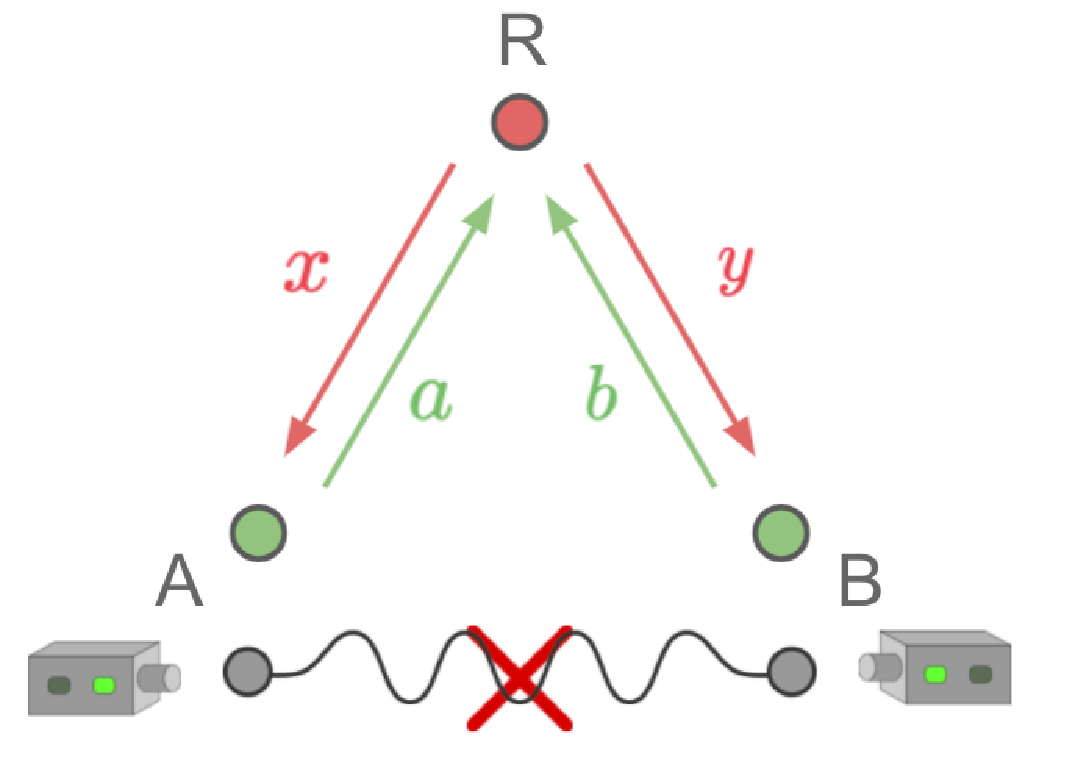
\includegraphics[width=0.8\textwidth]{lesson4/CHSH_broken_entanglement.pdf}
    \label{fig: 1}
    \begin{center}
        \caption{CHSH破壊された量子もつれ状態}
    \end{center}
\end{figure}
問題は\textit{AさんとBさんは持っている量子もつれを測定しなければならないことです}。これが前に説明したことあるとは思うんですけれども測定すると重ね合わせとそのもつれを破壊します。これがつぶしてしまうことになります。どうするのかは決めなきゃいけないんですよね。
もう一回CHSHゲームをやりたいなら新しい量子もつれの状態を作らなければ
なりません:
% insert new entangled connection
\begin{figure}[H]
   \centering
    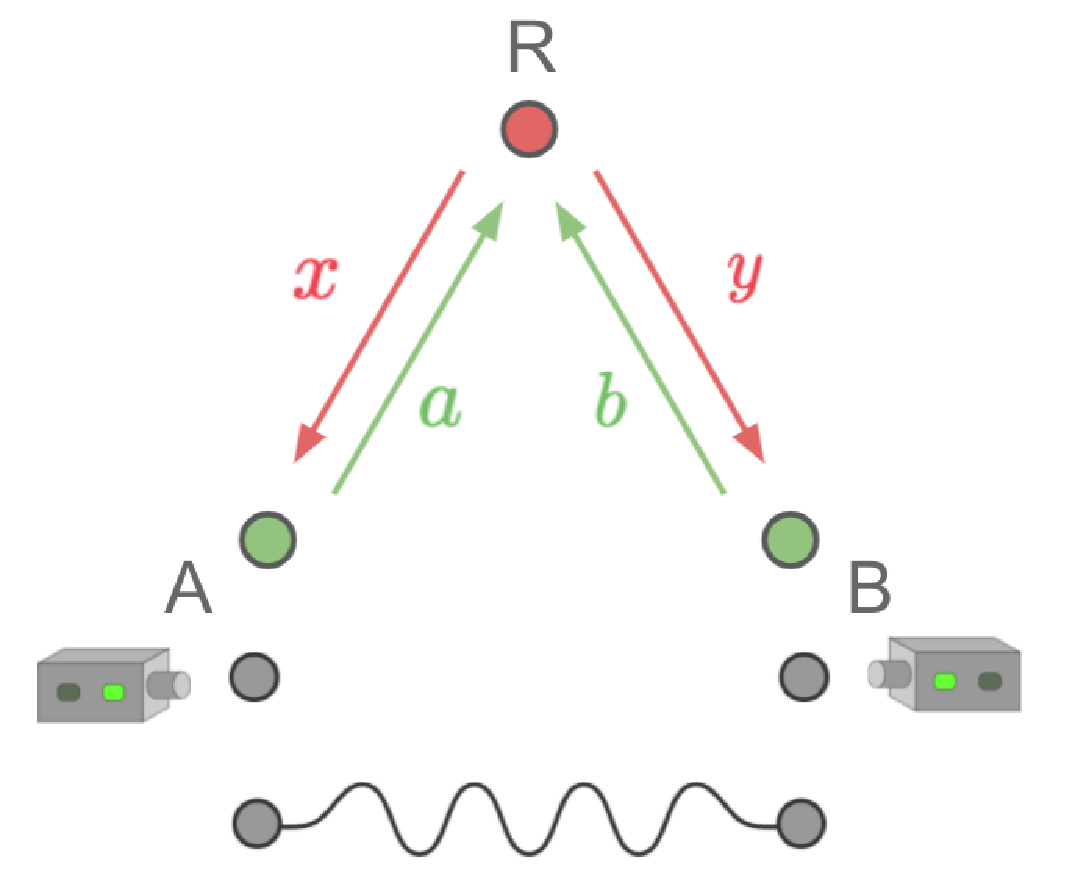
\includegraphics[width=0.8\textwidth]{lesson4/CHSH_new_connections.pdf}
    \label{fig: 1}
    \begin{center}
        \caption{CHSH量子もつれ状態}
    \end{center}
\end{figure}
つまりその量子状態を繰り返してやることにそれが繰り返してゲームを行うことができます。
\subsection{量子ネットワーク}
ていうわけはこの量子もつれは量子ネットワークの場合すごく重要なことなんですけれども、そうするとその状態を壊してしまうことによるとそれを繰り返して作ることがすごく重要な仕事です。それはネットワークの仕事の第一のポイントです。
じゃあちょっと
例を見てみましょう:
% network diagram
\begin{figure}[H]
   \centering
    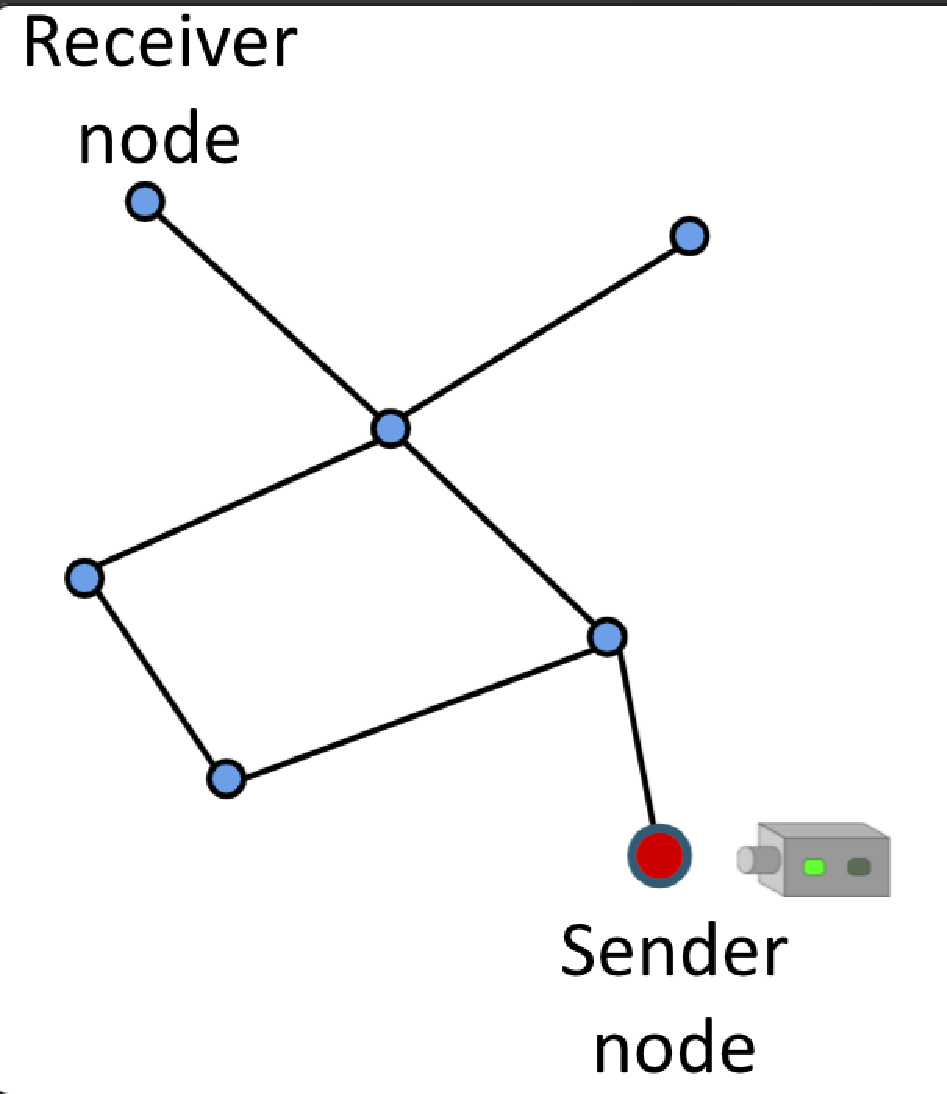
\includegraphics[width=0.8\textwidth]{lesson4/network_diagram.pdf}
    \label{fig: 1}
    \begin{center}
        \caption{量子ネットワーク:状態1}
    \end{center}
\end{figure}
例えばこういうネットワークが使ってる場合には
\textbf{丸がネットワークノード}として\textbf{線が量子もつれの状態}と考えていいんです。この場合には各キュービットじゃなくてそのノードには複数のキュービットが入っていると考えていいです。
じゃあこのネットワークの上には\textbf{sender node}と\textbf{receiver node}があってセンダーのノードは自分の持っているビットの量子状態をレシーバーに送りたい。じゃあどうすればいいでしょう。

これは\textbf{量子テレポーテーション}、今度のレッスンにはテレポーテーションを数学的に見てみますけれどもこの場合にはちょと定性的に説明するとまあテレポーテーションとしては持っているキュービットをこっちからあっちまで
転送することです。ですがそうすると量子もつれが
消えてしまいます。消費します。これがまあ量子もつれの消費者にはなるんでしょ。例えばセンダーがその状態をもつれを測定すると
使って持っている赤いキュービットを自分のところから次のステップまで転送してて繰り返して、それが1つ目のステップ先のノード
が自分で測定して、それを使って赤いキュービットの赤い状態を
転送することができて、もう一回繰り返してその3つ目は使ってreceiver
nodeつまりデスティネーションにはその状態が届きます:
\begin{figure}[H]
  \centering
  \begin{minipage}[b]{0.3\textwidth}
    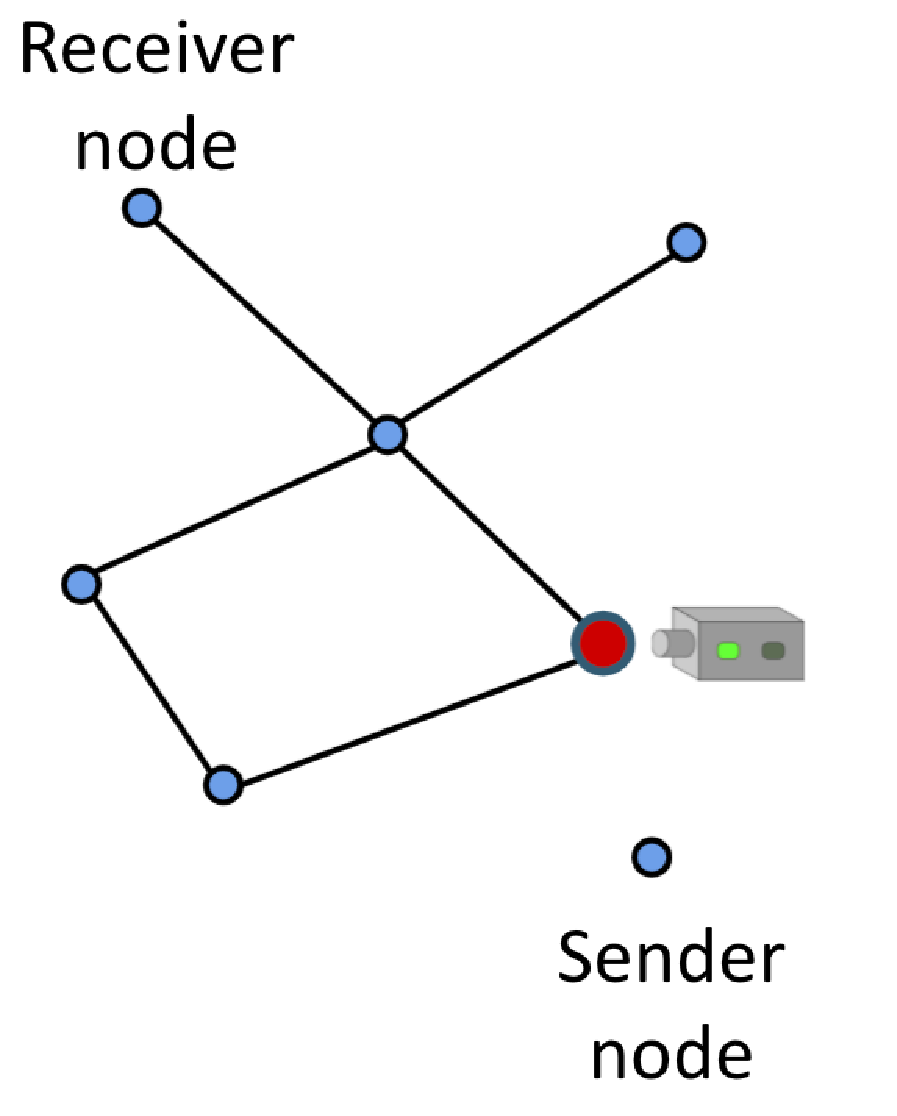
\includegraphics[width=\textwidth]{lesson4/network_state2.pdf}
    \caption{状態2}
  \end{minipage}
  \hfill
  \begin{minipage}[b]{0.3\textwidth}
    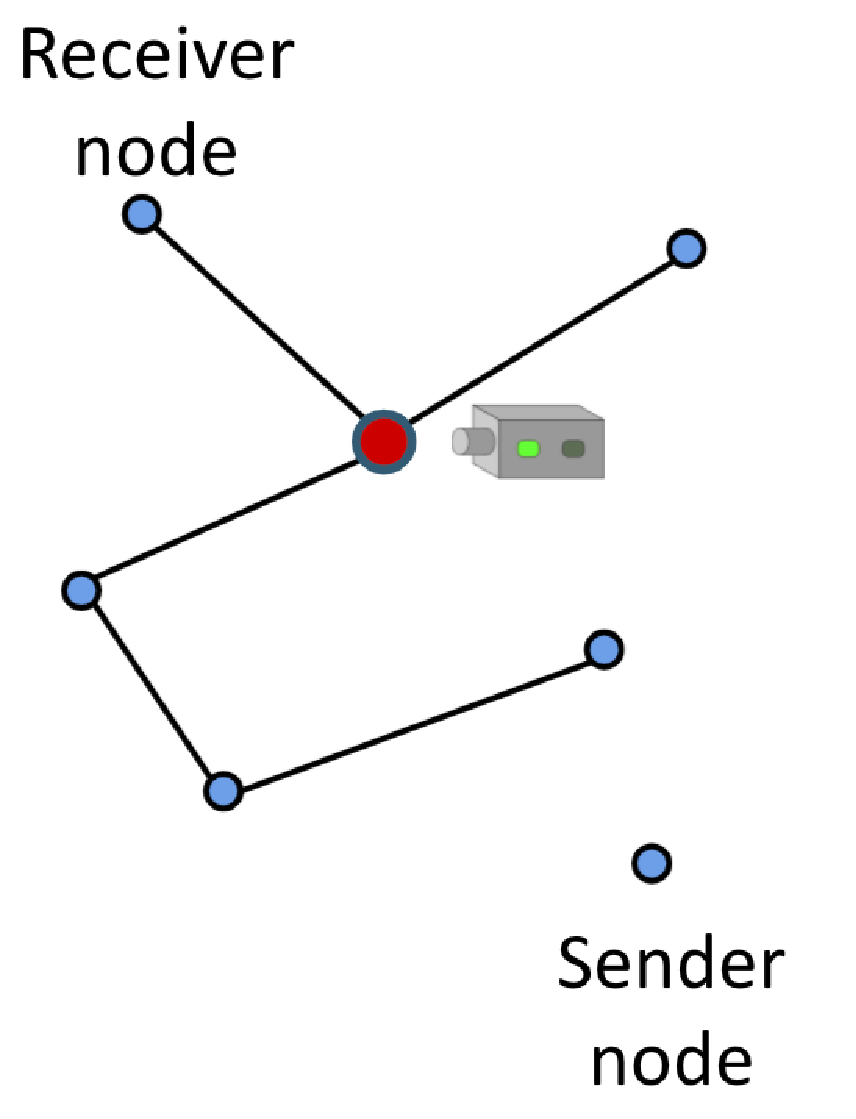
\includegraphics[width=\textwidth]{lesson4/network_state3.pdf}
    \caption{状態3}
  \end{minipage}
  \hfill
  \begin{minipage}[b]{0.3\textwidth}
    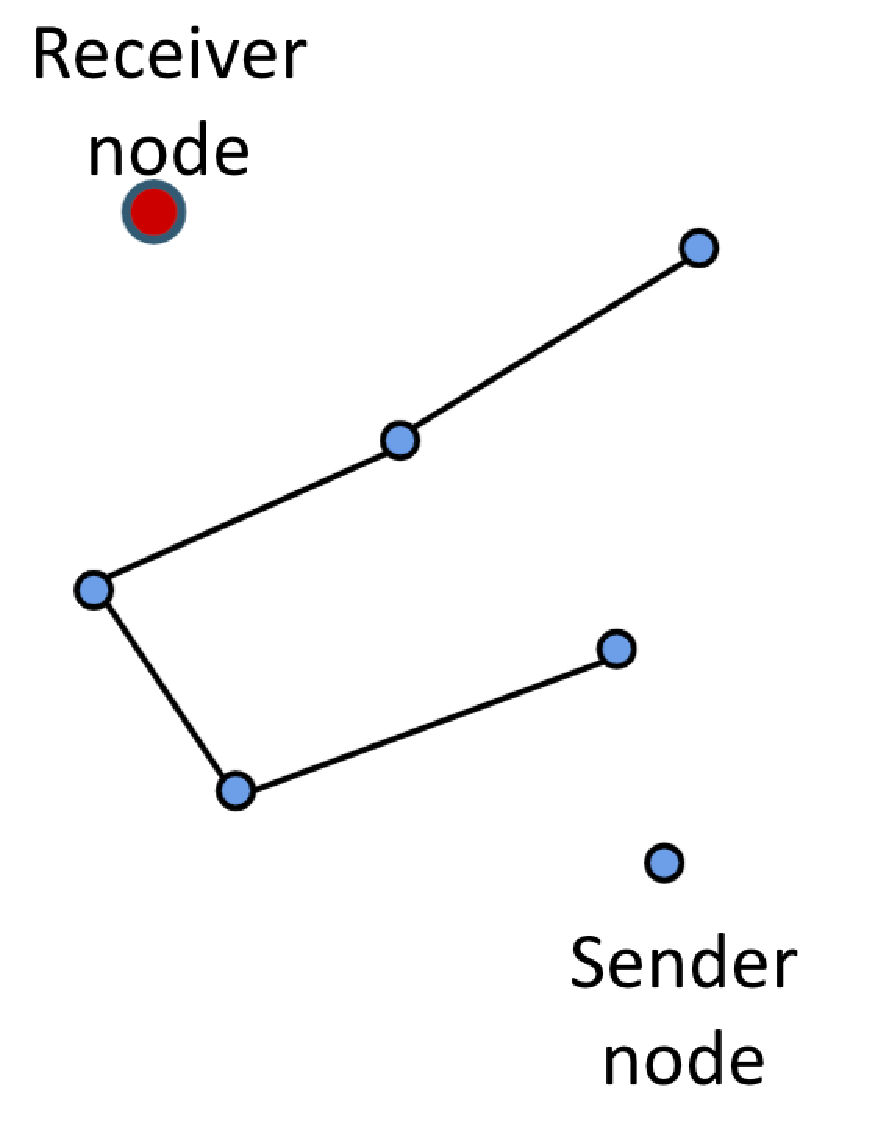
\includegraphics[width=\textwidth]{lesson4/network_state4.pdf}
    \caption{状態4}
  \end{minipage}
\end{figure}
ですがそうすると見たとおりでその線は無くなってってるでしょう。量子もつ
れがなくなってたんですがそれは消費されてしまってもう一回データを
送りたい場合があるとその量子もつれを作らなければ
ならない。それが連続で繰り返す。
ことそれがネットワークの重要な仕事です。

これが量子技術の「燃料」と思うんですけどまあ資源あるいは使えることなんですが、量子もつれの長所と言えば:
\begin{enumerate}
    \item 量子もつれ状態を使うと、古典的以上の性能や古典では存在しない機能を実装することができる。
    \item これが量子ネットワークを作る目的なんですけれども、量子もつれが消費資源になりますからその作ることは繰り返すことになります。
    \item 量子もつれを作るプロセスが速さと効率とフィデリティとかいろんな状態についてはそれがすごく重要なポイントになるんです。
\end{enumerate}
\iffalse
この量子もつれをうまく使うと古典的な世界にはない機能が行うことは
できます。
\fi

